\documentclass[12pt]{article}
\usepackage{fullpage,mathpazo,amsfonts,nicefrac}

\usepackage{kpfonts}
%\usepackage{fontspec}
%\setmainfont{Hoefler Text}

\usepackage{media9}

\usepackage{graphicx}

\usepackage{pgfplots}
\usepackage{pgfplotstable}
\usepackage{tikz}
\usetikzlibrary{arrows,automata,mindmap,shapes,positioning,patterns,snakes,calc}

\pgfplotsset{every x tick label/.append style={font=\small, yshift=0.2ex}}
\pgfplotsset{every y tick label/.append style={font=\small, xshift=0.2ex}}

\usepackage{multirow}
\makeatletter
\def\hlinew#1{%
  \noalign{\ifnum0=`}\fi\hrule \@height #1 \futurelet
   \reserved@a\@xhline}
\makeatother

\usepackage{amsmath,amsthm,mathrsfs,bm}
\usepackage{amssymb}% math symbols
\usepackage{mathtools}
\DeclarePairedDelimiter{\ceil}{\lceil}{\rceil}
\DeclarePairedDelimiter{\floor}{\lfloor}{\rfloor}

\numberwithin{table}{section}

\usepackage{hyperref}
\hypersetup{
    colorlinks=true,
    linkcolor=blue,
    filecolor=magenta,
}
\usepackage{color}

% color
\definecolor{marron}{RGB}{60,30,10}
\definecolor{darkblue}{RGB}{0,0,80}
\definecolor{lightblue}{RGB}{80,80,80}
\definecolor{darkgreen}{RGB}{0,80,0}
\definecolor{darkgray}{RGB}{0,80,0}
\definecolor{darkred}{RGB}{80,0,0}
\definecolor{shadecolor}{rgb}{0.97,0.97,0.97}

\newtheorem{theorem}{Theorem}[section]
\newtheorem{lemma}{Lemma}[section]
\newtheorem{definition}{Definition}[section]
\newtheorem{axiom}{Axiom}[section]
\newtheorem{property}{Property}[section]
\newtheorem{proposition}{Proposition}[section]
\newtheorem{corollary}{Corollary}[section]
\newtheorem{condition}{Condition}[section]
\newtheorem{conclusion}{Conclusion}[section]
\newtheorem{assumption}{Assumption}[section]
\newtheorem{remark}{Remark}[section]
\newtheorem{problem}{Problem}[section]
\newtheorem{solution}{Solution}[section]

\renewcommand{\emptyset}{\varnothing}
\DeclareMathOperator*{\argmax}{\mathrm{\arg\max}}
\DeclareMathOperator*{\argmin}{\mathrm{\arg\min}}
\DeclareMathOperator*{\arginf}{\mathrm{\arg\inf}}
\DeclareMathOperator*{\argsup}{\mathrm{\arg\sup}}
\DeclareMathOperator{\sgn}{\mathrm{sign}}
\DeclareMathOperator{\ind}{\mathrm{I}}
\DeclareMathOperator{\complex}{\mathrm{O}}
\DeclareMathOperator{\diag}{\mathrm{diag}}
\DeclareMathOperator{\prob}{\mathrm{Pr}}
\DeclareMathOperator{\E}{\mathrm{E}}
\DeclareMathOperator{\var}{\mathrm{var}}
\DeclareMathOperator{\corr}{\mathrm{corr}}
\DeclareMathOperator{\cov}{\mathrm{cov}}
\DeclareMathOperator{\rand}{\mathrm{rand}}
\DeclareMathOperator{\vect}{\textit{vec}}
\DeclareMathOperator{\rank}{\textit{rank}}
\DeclareMathOperator{\tr}{\textit{tr}}

\newcommand{\N}{\mathbb{N}}
\newcommand{\Z}{\mathbb{Z}}
\newcommand{\Q}{\mathbb{Q}}
\newcommand{\R}{\mathbb{R}}

% Useful for algorithms
\newcommand{\alg}[1]{\textsc{\bfseries \footnotesize #1}}

% For derivatives
\newcommand{\deriv}[1]{\frac{\mathrm{d}}{\mathrm{d}x} (#1)}

% For partial derivatives
\newcommand{\pderiv}[2]{\frac{\partial}{\partial #1} (#2)}

% Integral dx
\newcommand{\dx}{\mathrm{d}x}

\renewcommand{\figurename}{Fig.}
\renewcommand{\baselinestretch}{1.5}
\setlength{\parskip}{0.5em}

\usepackage{algpseudocode,algorithm,algorithmicx}
\newcommand*\Let[2]{\State #1 $\gets$ #2}
\renewcommand{\algorithmicrequire}{\textbf{Input:}}
\renewcommand{\algorithmicensure}{\textbf{Output:}}

\newenvironment{affiliations}{
    \setcounter{enumi}{1}
    \setlength{\parindent}{0in}
    \slshape\sloppy
    \begin{list}{\upshape$^{\arabic{enumi}}$}{
        \usecounter{enumi}
        \setlength{\leftmargin}{0in}
        \setlength{\topsep}{0in}
        \setlength{\labelsep}{0in}
        \setlength{\labelwidth}{0in}
        \setlength{\listparindent}{0in}
        \setlength{\itemsep}{0ex}
        \setlength{\parsep}{0in}
        }
    }{\end{list}\par\vspace{12pt}}

\renewcommand{\thefigure}{\arabic{figure}}
\renewcommand{\thesection}{\arabic{section}}
\renewcommand{\thetable}{\arabic{table}}
\renewcommand{\theequation}{\arabic{equation}}

\newcommand\jch[1]{{\color{red} \footnote{\color{red}JCH: #1}} }

\usepackage{cite}
\makeatletter
% remove the parenthesis
\renewcommand{\@biblabel}[1]{#1.}
\makeatother

\usepackage[comma,super,sort&compress]{natbib}

\setlength\parindent{0em}

\title{Speed Prediction from Taxi Trajectory Data}

\author{Chunheng Jiang}

\begin{document}

\maketitle
\noindent

%\begin{affiliations}
% \item Department of Computer Science, Rensselaer Polytechnic Institute, Troy, NY 12180.
%\end{affiliations}

\section*{Problem}
We are given a trajectory data of DiDi Express and DiDi Premier drivers within the Second Ring Road of Xi'An City. 
All track points are bound to physical roads with resolution about 2-4 seconds. The problem is to predict the average speed of all vehicles running on a segment of road (either north or south bound) at specific time. 

\section*{Data Preprocessing}
Each day contains millions records, and each record contains five columns: driver id, order id, timestamp, longitude, and latitude. Both driver id and order id are encrypted and anonymized with long strings. To reduce memory usage, we re-encode these ids as integers. As a result, file size will shrink from 2.2G to 1.0G. The unix timestamp can be converted into readable format, such that accompanied with the location we can calculated the average speed of the vehicle at given time. To compute the distance between a pair of longitude and latitude, we are required to call eviltransform\footnote{\href{https://github.com/googollee/eviltransform}{https://github.com/googollee/eviltransform}} using the same coordinate system.

There are 18,635 drivers, 111,541 trip orders, 86,495 different timestamps, and 16,224 different locations. To have an overview of the data, we examine the records distribution of each trip order. As seen from Fig.~\ref{fig:recordsperorder}, around 100 trip orders have only one record entry in the trajectory data, 120 trip orders have 10 records in each order, and majority of the records have several records tracked.

\begin{figure}[!h]
\centering
\includegraphics[width=\textwidth]{figs/RecordsPerOrder}
\caption{\textbf{Records distribution per order.} The $x-$axis is the possible number of records in a trip order, and $y-$axis is the number of orders with specific number of recording entries.} 
\label{fig:recordsperorder}
\end{figure}

\section*{Coordinate Systems and Timezone}
There are several different coordinate systems in spatial data processing, e.g. cartography, geodesy, and satellite navigation. As shown in Fig.~\ref{fig:roadsection}, OpenStreetMap\footnote{\href{https://www.openstreetmap.org/}{https://www.openstreetmap.org/}} uses the WGS-84 coordinate system (a.k.a World Geodetic System), but Google map uses GCJ-02 coordinate system (a.k.a Mars coordinate) for Chinese users. Therefore, it requires a conversion from one system to another to visualize the trajectories on Google map.

\begin{figure}[!h]
\centering
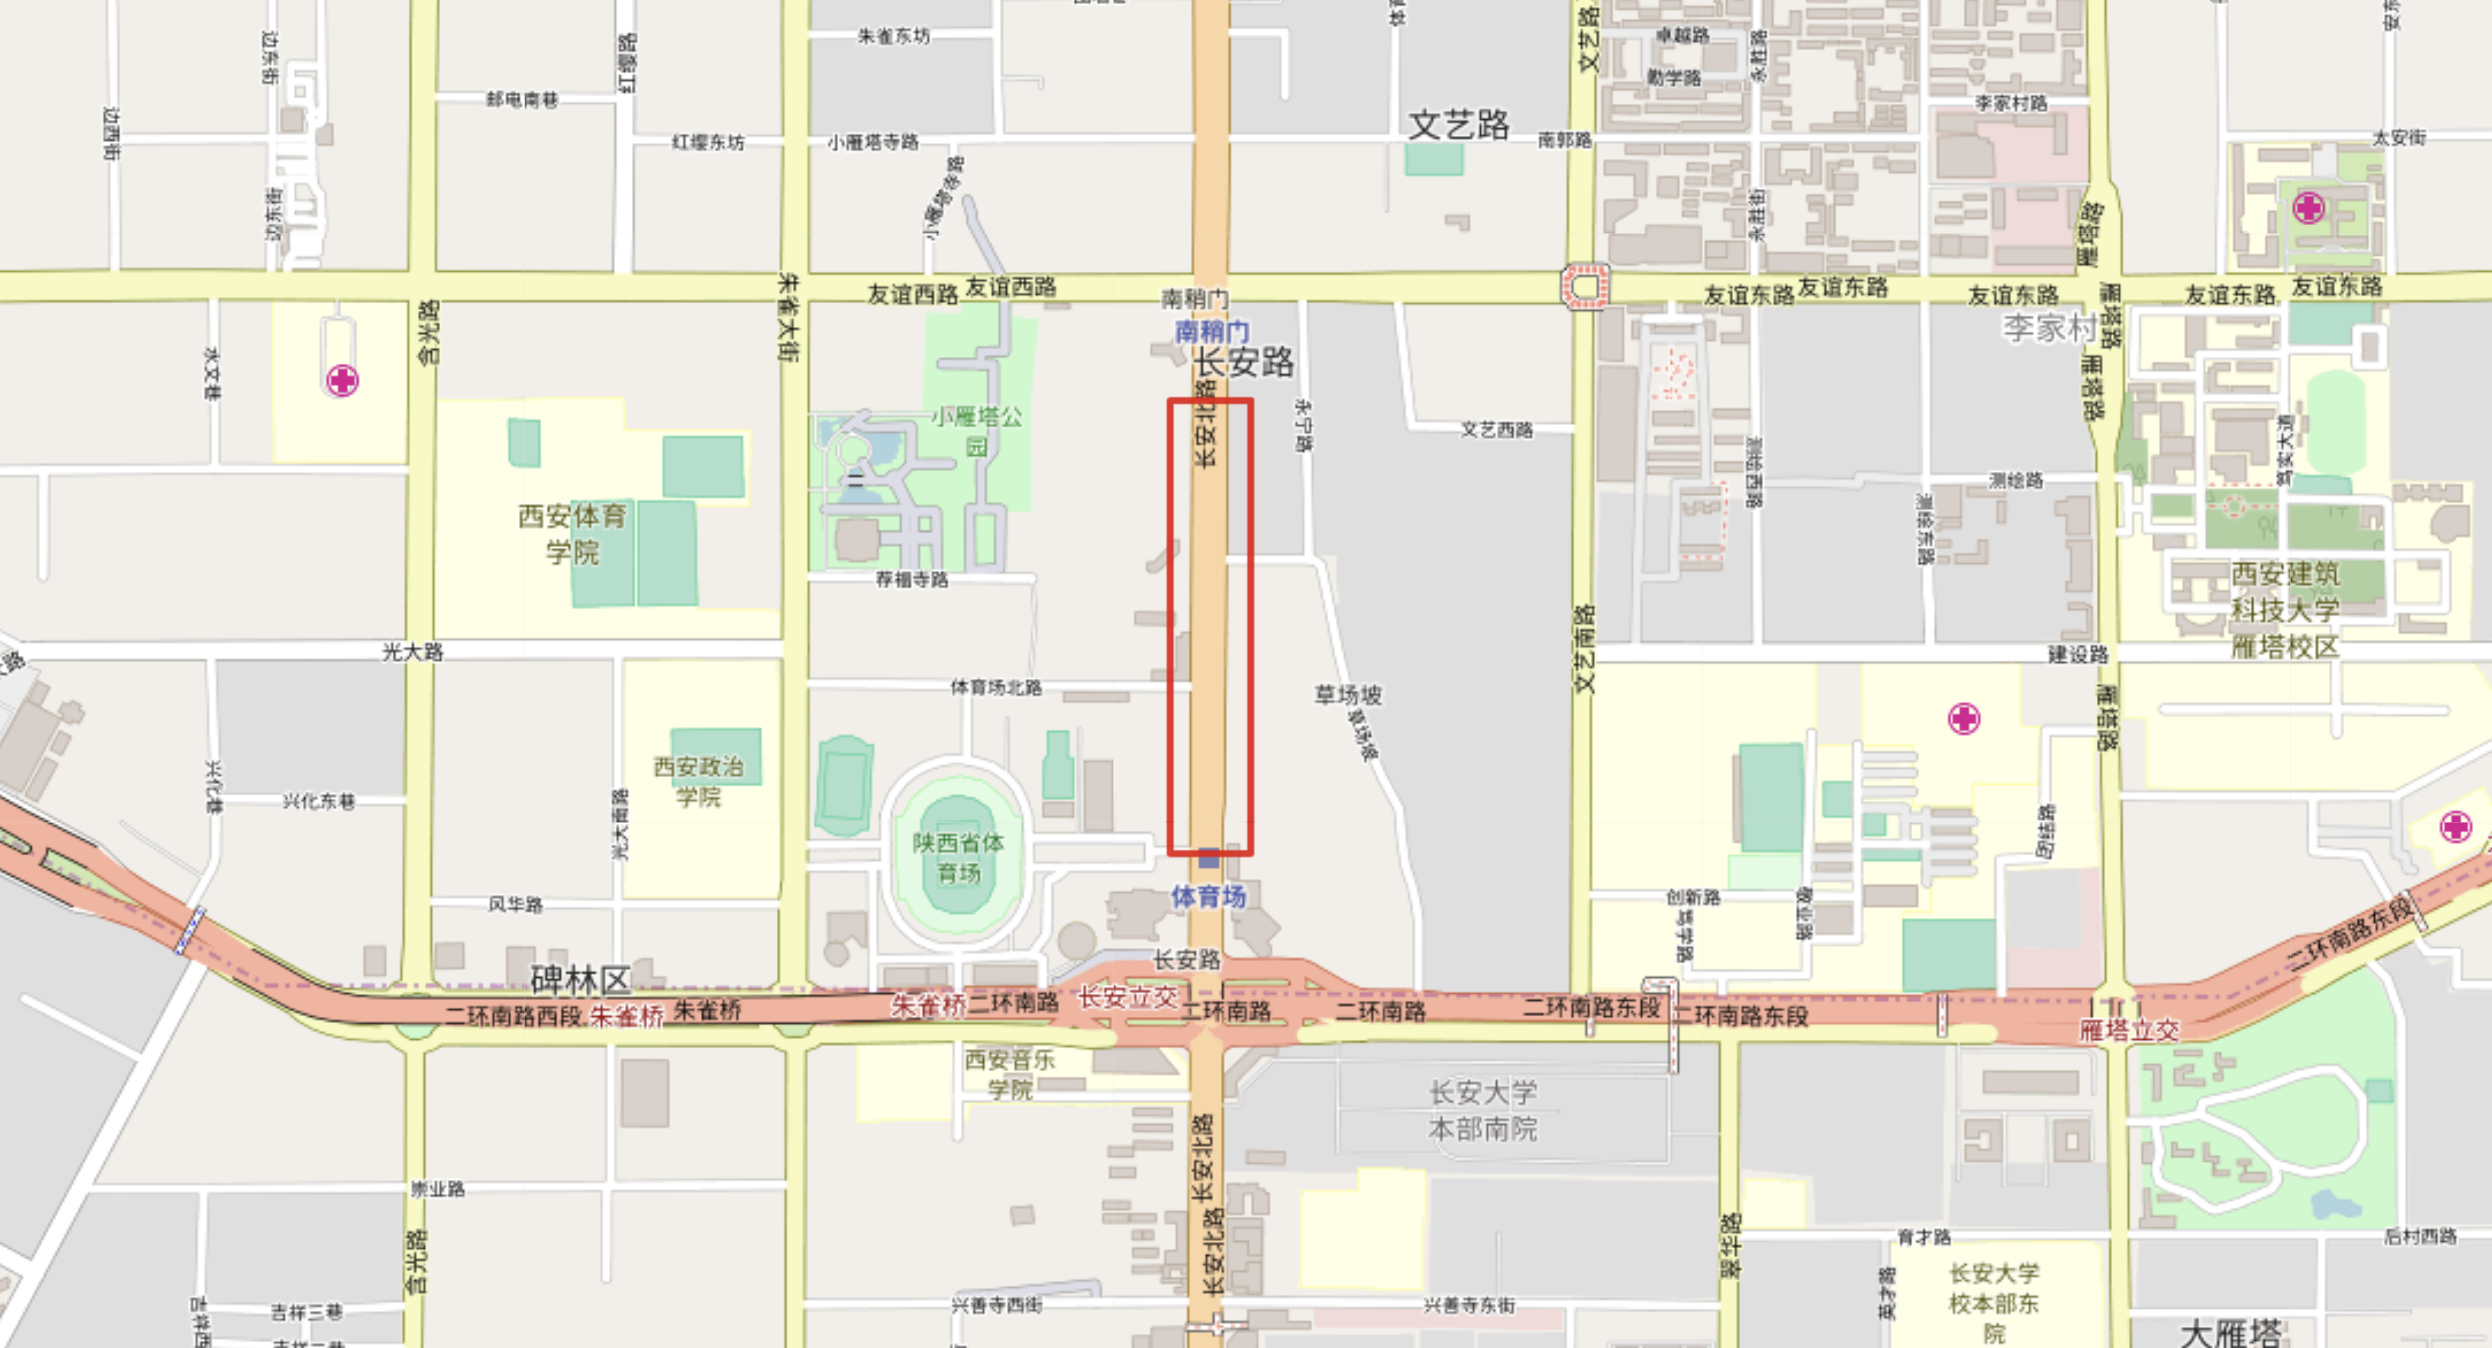
\includegraphics[width=\textwidth]{figs/XiAn}
\caption{\textbf{Road section to be predict.} The road section selected for prediction. The average driving speeds of all vehicles driving towards both north bound (latitude increasing) and south bound in every 5 minute are required to predict.} 
\label{fig:roadsection}
\end{figure}

%\clearpage
The road section in question (see red rectangular in Fig.~\ref{fig:roadsection}) is defined by four corners in counter-clockwise:
\begin{itemize}
\item Point 1 (upper-right): 34.241, 108.943
\item Point 2 (upper-left): 34.241, 108.9415
\item Point 3 (lower-left): 34.234, 108.9415
\item Point 4 (lower-right): 34.234, 108.943
\end{itemize}

Another important aspect is the underlying timezone, which is supposed to be GMT+8. Therefore, we need to convert the timestamp with specific timezone, i.e. Asia/Shanghai. The prediction will be made based on the assumption that the drivers in the extra day exactly replicates what they behaved in previous day. The trajectory file have a time range from 00:01:37 Dec 1, 2016 to 00:03:55 Dec 2, 2016. Also, the missing average speeds for north bound traffic are morning peak hours from 06:00:05 to 10:55:05, afternoon peak hours from 16:00:05 to 20:55:05, while for south bound traffic the missing average speeds in morning peak hours starts from 06:00:04 to 10:55:04, afternoon peak hours from 16:00:04 to 20:55:04.

\section*{Data Preprocessing}
To predict the missing components, we need to recovery the average speeds during the same time interval based on the known trajectories and the given average speeds in other time intervals. However, the given trajectories maybe do not contribute any useful information when they do not hit the specific road section. To estimate the average speeds in the given road section, we are required to identify all trips that fall into the road section based on the latitude and longitude information. 

The first step will be data filtering, we are figuring out the trajectories that have overlap region with the road section set by the rectangular. We can imagine the data will become sparser, and many trajectories will definitely been truncated. Some of the data points may be useful even though not included by the specific region. For example, the down-stream or up-stream traffic, the entering or exit ramps.

\bibliographystyle{naturemag}
\bibliography{ref}

\end{document}
